\documentclass[runningheads]{llncs}

\usepackage{amsmath, amssymb}
\usepackage{enumitem}
\usepackage{wrapfig}
\usepackage{tikz}

\usetikzlibrary{shapes, arrows}
\usetikzlibrary{automata}
\usetikzlibrary{positioning}
\usetikzlibrary{lindenmayersystems}

\newcommand{\east}{{\ensuremath \to}}
\newcommand{\se}{{\ensuremath \searrow}}

\DeclareMathOperator*{\argmin}{arg\,min}

\title{Towards the Algorithmic Molecular Self-Assembly of Fractals by Cotranscriptional Folding\thanks{This work is in part supported by JST Program to Disseminate Tenure Tracking System, MEXT, Japan, No.~6F36 and by JSPS KAKENHI Grant-in-Aid for Young Scientists (A) No.~16H05854 to S.~S.}}
\titlerunning{Algorithmic Self-Assembly of Fractals by Cotranscriptional Folding}
\author{
Yusei Masuda \and 
Shinnosuke Seki\thanks{Corresponding author} \and 
Yuki Ubukata
}
\institute{
Department of Computer and Network Engineering, 
The University of Electro-Communications, 
1-5-1, Chofugaoka, Chofu, Tokyo, 1828585, Japan 
\email{s.seki@uec.ac.jp}
}

\begin{document}

\maketitle

\begin{abstract}
RNA cotranscriptional folding has been just experimentally proven capable of self-assembling a rectangular tile at nanoscale {\it in vivo} (RNA origami). 
%The oritatami system (OS) is a novel computational model of cotranscriptional folding. 
We initiate the theoretical study on the algorithmic self-assembly of shapes by cotranscriptional folding using a novel computational model called the oritatami system. 
We propose an oritatami system that folds into an arbitrary finite portion of the Heighway dragon fractal, also-known as the paperfolding sequence $P = {\rm RRLRRLLR} \cdots$. 
The $i$-th element of $P$ can be obtained by feeding $i$ in binary to a 4-state DFA with output (DFAO). 
We implement this DFAO and a bit-sequence bifurcator as modules of oritatami system. 
Combining them with a known binary counter yields the proposed system. 
\end{abstract}

%--------------------------------------------------------------------------------------------------------
	\section{Introduction}
%--------------------------------------------------------------------------------------------------------

An RNA sequence, over nucleotides of four kinds {\tt A}, {\tt C}, {\tt G}, {\tt U}, is synthesized (\textit{transcribed}) from its template DNA sequence over {\tt A}, {\tt C}, {\tt G}, {\tt T} nucleotide by nucleotide by an RNA polymerase (RNAP) enzyme according to the one-to-one mapping ${\tt A} \to {\tt U}$, ${\tt C} \to {\tt G}$, ${\tt G} \to {\tt C}$, and ${\tt T} \to {\tt A}$ (for details, see, e.g., \cite{AJLMRRW2014}). 
The yield, called \textit{transcript}, starts folding immediately after it emerges from RNAP. 
This is the \textit{cotranscriptional folding} (see Fig.~\ref{fig:rna_origami}). 
Geary, Rothemund, and Andersen have recently demonstrated the capability of cotranscriptional folding to self-assemble an RNA molecule of an intended shape at nano-scale \cite{GearyRothemundAndersen2014}. 
They actually proposed an architecture of a DNA sequence whose transcript folds cotranscriptionally into an RNA tile of specific rectangular shape highly likely \textit{in vitro}. 

\begin{figure}[tb]
\centering
\includegraphics[width=0.8\linewidth]{Figs/rna_origami.pdf}
\caption{RNA cotranscriptional folding. 
An RNA polymerase attaches to a template DNA sequence (gray spiral), scans it through, and synthesizes its RNA copy. 
The RNA sequence begins to fold upon itself immediately as it emerges from polymerase. 
}
\label{fig:rna_origami}
\end{figure}

Algorithms and computation are fundamental to molecular self-assembly as illustrated in an enormous success of their use in DNA tile self-assembly (see, e.g., \cite{Doty2012,Patitz2016,WinfreePhD} and references therein). 
%The concepts of computation and algorithms are yet to be as much utilized in the self-assembly of shapes by cotranscriptional folding as in the DNA tile self-assembly, where for example 
The Sierpinski triangle fractal was algorithmically self-assembled even \textit{in vitro} from coalescence of DNA tiles that compute XOR \cite{RothemundPapadakisWinfree2004}. 
Cotranscriptional folding exhibits highly sophisticated computational and algorithmic behaviors as well. 
Indeed, fluoride riboswitches in \textit{Bacillus cereus} bacteria cotranscriptionally fold into a terminator stem or do not, in order to regulate gene expression \cite{WaStYuLiLu2016}. %depending on ligand concentration \cite{WaStYuLiLu2016}. 
This is just one example but should be enough to signify both the context-sensitivity of cotranscriptional folding and shapes thus self-assembled. 
Geary et al.~have proved the capability of context-sensitivity to count in binary using a novel mathematical model of cotranscriptional folding called \textit{oritatami system} (abbreviated as OS) \cite{GeMeScSe2016}. 

%Cotranscriptional folding is in fact proved Turing-universal by the oritatami system \cite{GeMeScSe2015}. 
%The Turing-machine simulator is gigantic and intricate but oritatami systems have implemented basic computational devices such as binary counter \cite{GeMeScSe2016} as a module comparable in size to the gene expression regulator. 
%The binary counter module consists of half-adder components, which fold into one of possible four conformations depending on a 1-bit input and a 1-bit carry/non-carry encoded in their surroundings somehow. 
%It can be diverted as a copier for binary sequences by being fed with the non-carry. 
%They shall be reused in this paper. 

\begin{figure}[tb]
\centering
\begin{minipage}{0.4\linewidth}
\centering
\scalebox{0.7}{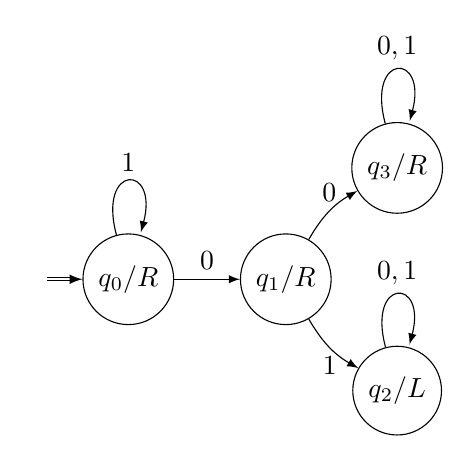
\begin{tikzpicture}[>=latex, node distance=2cm, initial text=, bend angle=15]
	\tikzstyle{every initial by arrow} = [->, double];

	\node [state, initial] (q_0)                        {$q_0/R$};
	\node [state]                     (q_1) [right of = q_0]  {$q_1/R$};
	\node [state]                     (q_2) [below right of = q_1] {$q_2/L$};
	\node [state]                     (q_3) [above right of = q_1] {$q_3/R$};

	\path [->] (q_0) edge [right] node [above]              {$0$}                 (q_1)
         		         edge [loop above] node [above]             {$1$}               ()
         			   (q_1) edge [bend left] node [above]             {$0$}                 (q_3)
         		         edge [bend right] node [below]             {$1$}              (q_2)
         			   (q_2)  edge [loop above] node [above]             {$0,1$}               ()
         			   (q_3)  edge [loop above] node [above]             {$0,1$}               ();
\end{tikzpicture}}
\end{minipage}
\begin{minipage}{0.05\linewidth}
\ \\
\end{minipage}
\begin{minipage}{0.5\linewidth}
\centering
\scalebox{0.03}{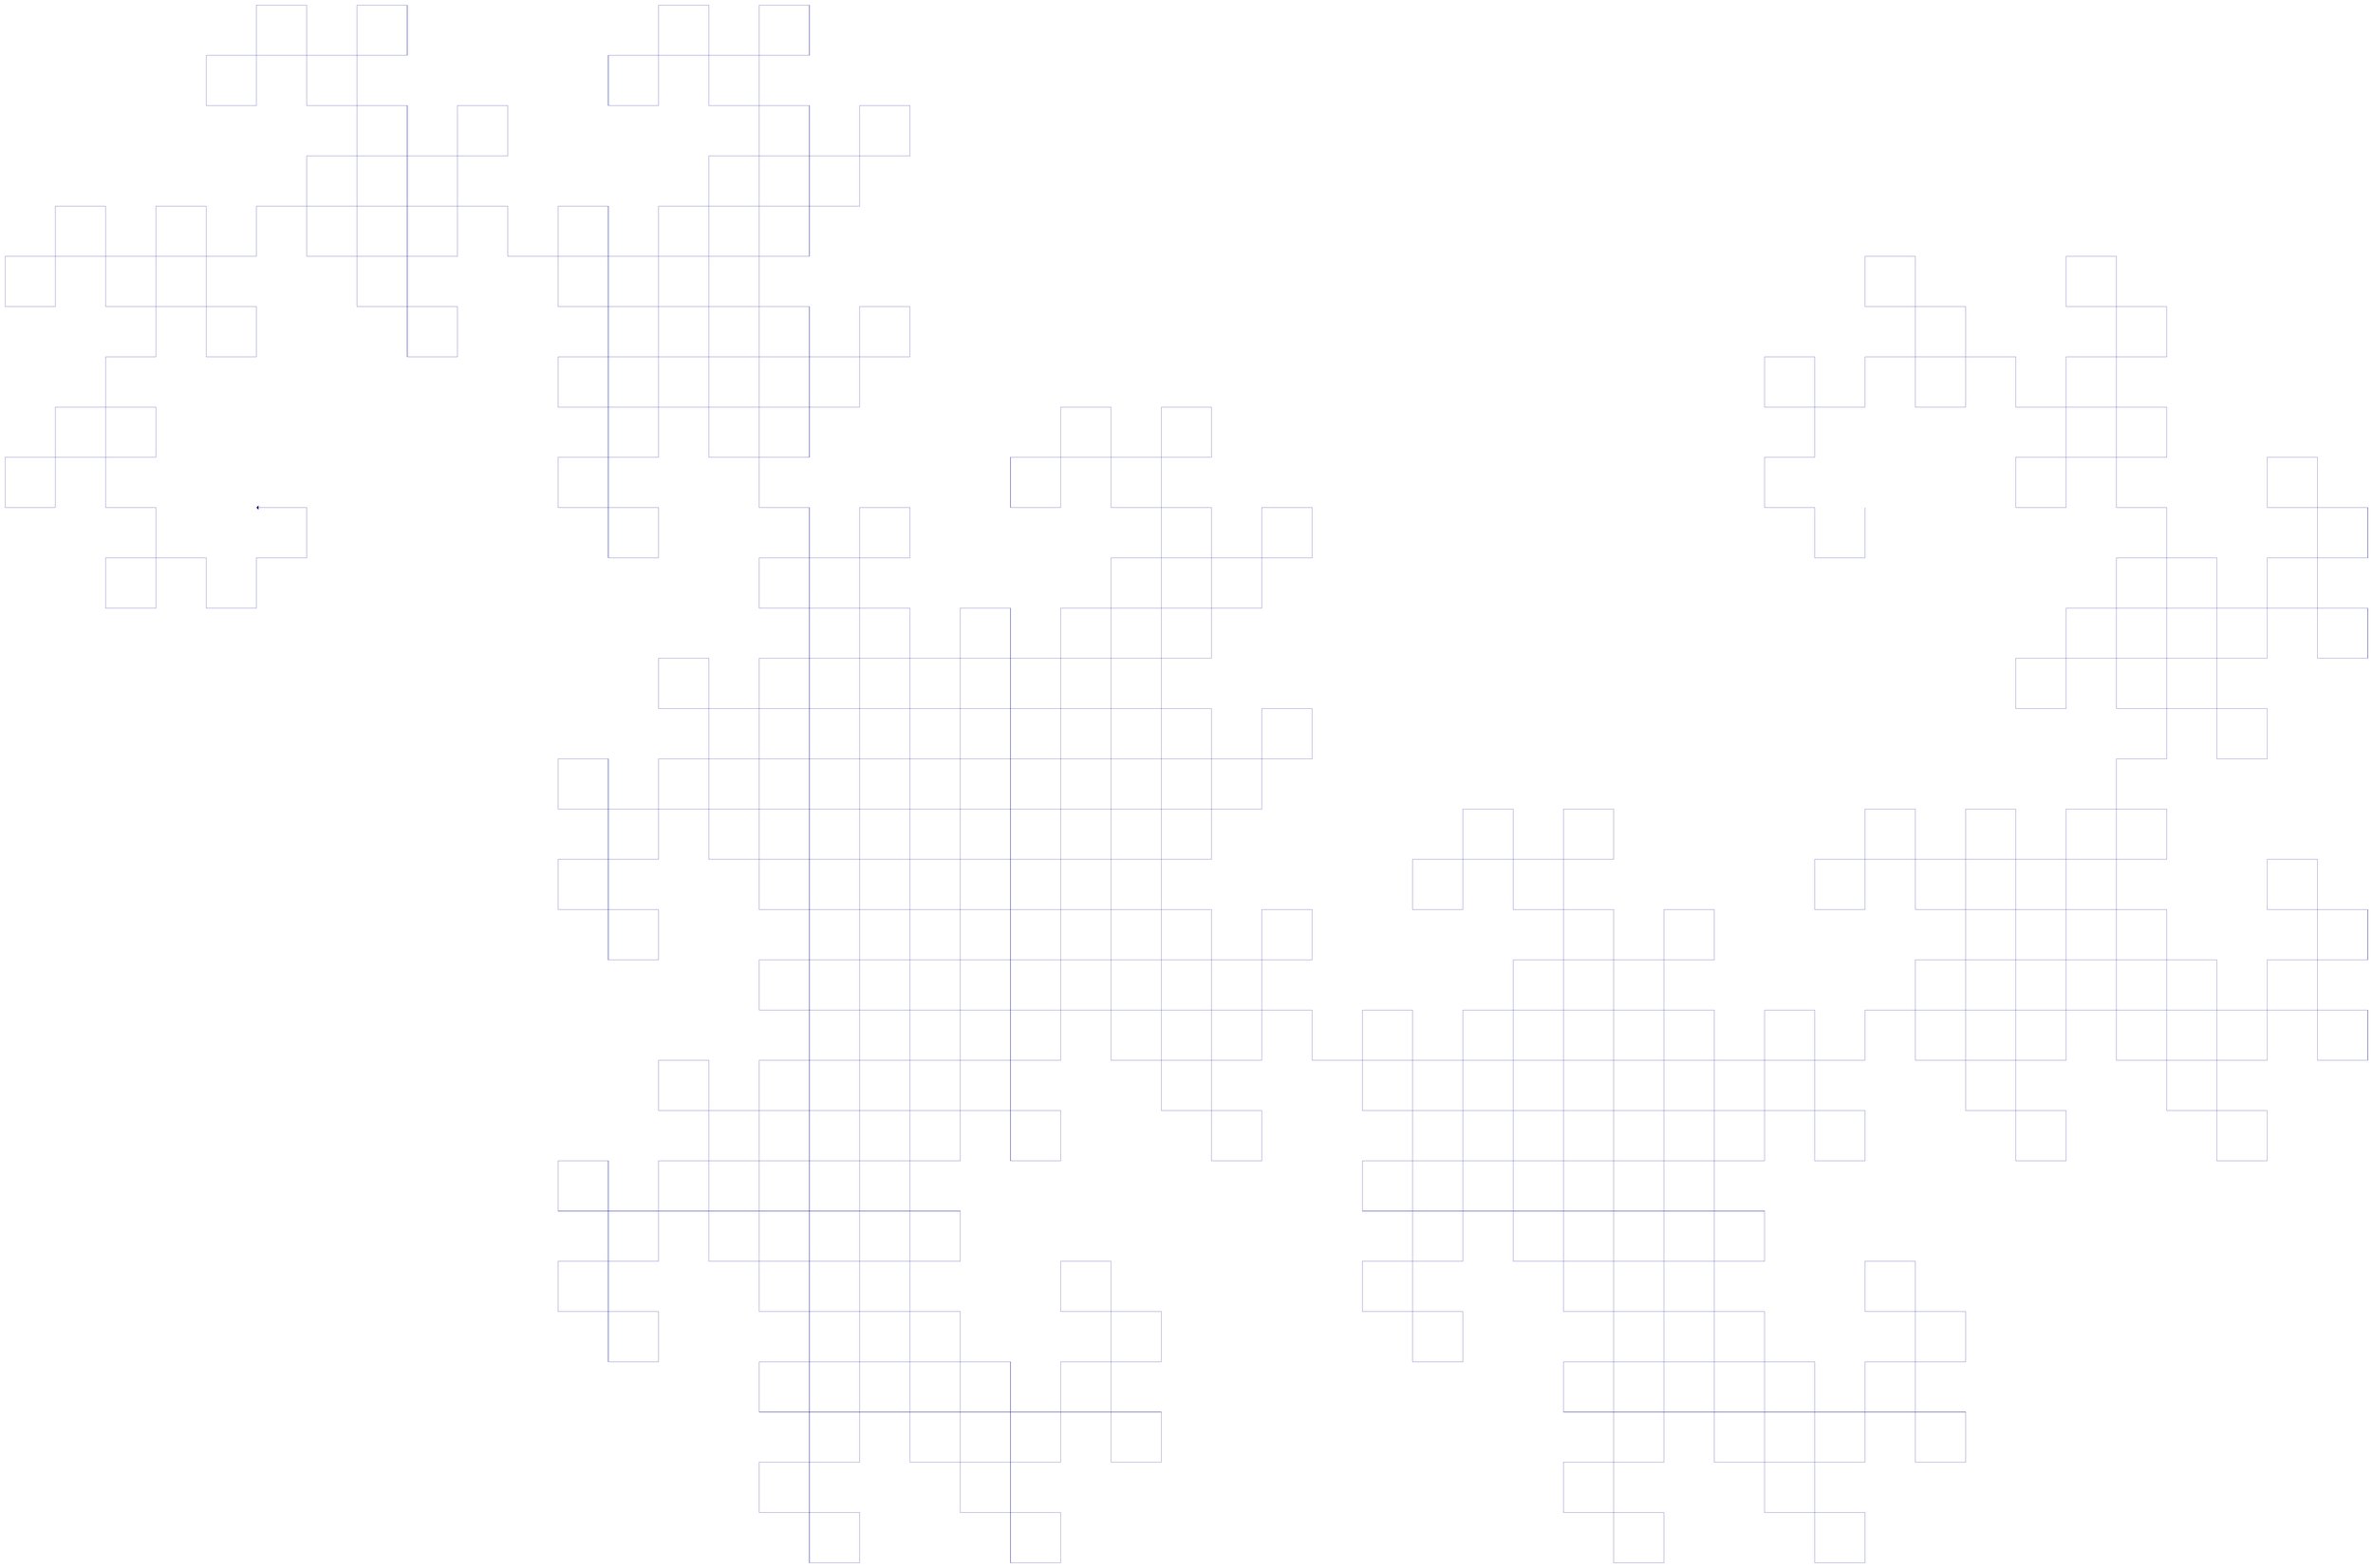
\begin{tikzpicture}
  \draw[blue!50!black,rotate=270,l-system={rule set={X->X-YF,Y->FX+Y},
  step=100pt,angle=90,axiom=FX,order=10},-triangle 90] l-system;
\end{tikzpicture}}
\end{minipage}
\caption{
%Heighway dragon. 
(Left) DFAO to output the direction (L/R) of $i$-th turn of the Heighway dragon given $i \ge 0$ in binary from the LSB. 
(Right) The first $2^{10}{-}1$ turns of the dragon. 
}
\label{fig:heighway_dragon}
\end{figure}

We shall initiate theoretical study on algorithmic self-assembly of shapes by cotranscriptional folding using oritatami system. 
Sierpinski triangle would allow our study to borrow rich insights from the DNA tile self-assembly. 
However, in order to cut directly to the heart of algorithmic self-assembly by cotranscriptional folding, shapes of choice should be traversable somehow algorithmically. 
One such way is to feed a turtle program (see \cite{AbelsondiSessa1981}) with an \textit{automatic sequence} as commands (drawing a line segment, rotation, etc.), whose $i$-th bit can be obtained by giving $i$ in binary from the least significant bit (LSB) to one DFA with output (DFAO) \cite{AlloucheShallit2003}.
Shapes thus describable include the Heighway dragon \cite{AlloucheShallit2003} and von Koch curve \cite{MaHoldener2005}. 
A DFAO for the Heighway dragon is illustrated in Fig.~\ref{fig:heighway_dragon}. 
It outputs the following sequence, given $i = 0, 1, 2, \ldots$ in binary: 
%It is to read the binary representation of $i \ge 0$ from the LSB and outputs the $i$-th direction $P[i]$ to turn (L or R) assigned to the state finally reached as follows: 
\[
%\begin{array}{cccrrrrc}
%i 	&=& 0 &  2 & 6 & 14 & 30 & \cdots \\
%P[i] 	&=& {\rm R} & {\rm RL} & {\rm RRLL} & {\rm RRRLLRLL} & {\rm RRRLRRLLLRRLLRLL} & \cdots.
%\end{array}
P 	= {\rm RRLRRLLRRRLLRLLRRRLRRLLLRRLLRLL} \cdots.
\]
(The notation $P$ is after its appellative \textit{paperfolding sequence} \cite{AlloucheShallit2003}.) 
For instance, given $i = 2$ in binary from the LSB as 01, the DFAO transitions as $q_0 \to q_1 \to q_2$ and hence $P[2] = {\rm L}$. 
%where only the values of $i$ at the end of the first five iterations are specified. 
A turtle should interpret an L (resp.~R) as ``move forward by unit distance and turn left (resp. right) 90 degrees.''
Any portion of the dragon can be represented by a factor of $P$; for instance, Fig.~\ref{fig:heighway_dragon} (Right) depicts the portion $P[0 .. 1022]$, i.e., the first $2^{10}-1$ turns of the dragon. 

%\begin{figure}[htb]
\begin{wrapfigure}{l}{0.57\linewidth}
\vspace*{-5mm}
\centering
\includegraphics[width=\linewidth]{Figs/6bit_heighway.pdf}
\caption{The portion $P[0 .. 62]$ of the Heighway dragon folded by the proposed oritatami system.}
\label{fig:heighway6_oritatami}
\vspace*{-5mm}
\end{wrapfigure}
%\end{figure}

In this paper, we propose a generic design of oritatami system for the algorithmic cotranscriptional folding of an arbitrary finite portion of the Heighway dragon. 
Fig.~\ref{fig:heighway6_oritatami} shows the portion $P[0 .. 62]$ thus folded (the dragon is slanted but this is because the OS operates on the triangular grid). 
The transcript is a repetition of three modules: a catenation of binary counters, DFAO module, and turning module. 
The counter is a technical modification of the one proposed in \cite{GeMeScSe2016} so that it increments a given count $i$ exactly by 1 while folding into a (red) line segment. 
%By being fed with carry exactly once, the catenation increments the count $i$ exactly by 1 while folding into a (red) line segment. 
At the end of the segment comes a DFAO module, which computes the turn direction $P[i]$ and propagates it alogn with the count $i$ to the next module for turn.  
A (green) L-shaped block is the turning module. 
It is a concatenation of three bit-sequence bifurcators, each of which folds into a rhombus, bifurcates $i$ leftward as well as rightward, and guides further folding according to the turning direction. 
%We shall implement the DFAO and turning modules and verify them. 

The generic design proves the next theorem (for terminologies, see Sect.~\ref{sect:preliminaries}). 

\begin{theorem}\label{thm:main}
	For any finite portion $P[i..j]$ of the Heighway dragon, there exist a scaling factor $c \in \mathbb{N}^+$ and a cyclic deterministic oritatami system of delay 3 and arity 3 that weakly folds into the $c$-rhombus scaling of $P[i..j]$. 
\end{theorem}

\noindent
A JavaScript program to run this OS is available at {\small {\tt https://wolves13.github.io}}. 

%--------------------------------------------------------------------------------------------------------
	\section{Preliminaries}
	\label{sect:preliminaries}
%--------------------------------------------------------------------------------------------------------

Let $\Sigma$ be a set of types of abstract molecules, or \textit{beads}, and $\Sigma^*$ be the set of finite sequences of beads. 
A bead of type $a \in \Sigma$ is called an $a$-bead. 
Let $w = b_1 b_2\cdots b_n \in \Sigma^*$ be a string of length $n$ for some integer $n$ and bead types $b_1, \ldots, b_n \in \Sigma$.
The \textit{length} of $w$ is denoted by $|w|$, that is, $|w| = n$. 
For two indices $i,j$ with $1\leq i \leq j \leq n$, we let $w[i..j]$ refer to the subsequence $b_i b_{i+1} \cdots b_{j-1} b_{j}$; if $i=j$, then we simplify $w[i..i]$ as $w[i]$.
For $k \ge 1$, $w[1..k]$ is called a \textit{prefix} of $w$. 

Oritatami systems fold their transcript, a sequence of beads, over the triangular grid graph $\mathbb{T} = (V, E)$ as suggested in Fig.~\ref{fig:glider} cotranscriptionally based on hydrogen-bond-based interactions (\textit{h-interactions} for short) which the system allow for between adjacent beads of particular types. 
A directed path $P = p_1 p_2 \cdots p_n$ in $\mathbb{T}$ is a sequence of \textit{pairwise-distinct} points $p_1, p_2, \ldots, p_n \in V$ such that $\{p_i, p_{i+1}\} \in E$ for all $1 \leq i < n$.
Its $i$-th point is referred to as $P[i]$. 

A \textit{conformation} $C$ is a triple $(P, w, H)$ of a directed path $P$ in $\mathbb{T}$, $w \in \Sigma^*$ of the same length as $P$, and a set of h-interactions $H \subseteq \{\{i,j\} \mid 1 \leq i, i+2 \leq j, \{P[i], P[j]\} \in E\}$.
This is to be interpreted as the sequence $w$ being folded in such a manner that its $i$-th bead $w[i]$ is placed on the $i$-th point $P[i]$ along the path and there is an h-interaction between the $i$-th and $j$-th beads if and only if $\{i, j\} \in H$. 
The condition $i+2 \leq j$ represents the topological restriction that two consecutive beads along the path cannot form an h-interaction between them.
A \textit{rule set} $\mathcal{H} \subseteq \Sigma \times \Sigma$ is a symmetric relation over the set of pairs of bead types, that is, for all bead types $a, b \in \Sigma$, $(a, b) \in \mathcal{H}$ implies $(b, a) \in \mathcal{H}$. 
An h-interaction $\{i, j\} \in H$ is \textit{valid with respect to $\mathcal{H}$}, or simply \textit{$\mathcal{H}$-valid}, if $(w[i], w[j]) \in \mathcal{H}$. 
This conformation $C$ is $\mathcal{H}$-valid if all of its h-interactions are $\mathcal{H}$-valid. 
%For an integer $\alpha \ge 1$, $C$ is \textit{of arity $\alpha$} if the maximum number of h-interactions per bead is $\alpha$, that is, if for any $k \ge 1$, $|\{i \mid (i, k) \in H)\}| + |\{j \mid (k, j) \in H\}| \le \alpha$ and this inequality holds as an equation of some $k$. 
For an integer $\alpha \ge 1$, $C$ is \textit{of arity $\alpha$} if it contains a bead that forms $\alpha$ h-interactions and no bead of $C$ forms more. 
By $\mathcal{C}_{\le \alpha}$, we denote the set of all conformations of arity at most $\alpha$.

Oritatami systems grow conformations by elongating them under their own rule set. 
Given a rule set $\mathcal{H}$ and an $\mathcal{H}$-valid finite conformation $C_1 = (P, w, H)$, 
we say that another conformation $C_2$ is an \textit{elongation of} $C_1$ \textit{by a bead} $b \in \Sigma$, written as $C_1 \xrightarrow{\mathcal{H}}_b C_2$, if $C_2 = (Pp, wb, H \cup H')$ for some point $p$ not along the path $P$ and set of h-interactions $H' \subseteq \left\{ \{i, |w|+1\} \bigm| 1\leq i < |w|, \{P[i], p\} \in E, (w[i], b) \in \mathcal{H}\right\}$, which can be empty.
Note that $C_2$ is also $\mathcal{H}$-valid.
This operation is recursively extended to the elongation by a finite sequence of beads as: 
for any conformation $C$, $C \xrightarrow{\mathcal{H}}^*_\lambda C$; 
and for a finite sequence of beads $w \in \Sigma^*$ and a bead $b \in \Sigma$,
a conformation $C_1$ is elongated to a conformation $C_2$ by $wb$,
written as $C_1 \xrightarrow{\mathcal{H}}^*_{wb} C_2$, if there is a conformation $C'$ that satisfies
$C_1 \xrightarrow{\mathcal{H}}^*_w C'$ and $C' \xrightarrow{\mathcal{H}}_b C_2$.

A finite \textit{oritatami system} (OS) is a 5-tuple $\Xi = (\mathcal{H}, \alpha, \delta, \sigma,w)$, where 
$\mathcal{H}$ is a rule set,
$\alpha$ is an arity, 
$\delta \geq 1$ is a parameter called the \textit{delay}, 
$\sigma$ is an initial $\mathcal{H}$-valid conformation of arity $\alpha$ called the \textit{seed}, upon which its finite \textit{transcript} $w \in \Sigma^*$ is to be folded by stabilizing beads of $w$ one at a time so as to minimize energy collaboratively with the succeeding $\delta -1$ nascent beads. 
The energy of a conformation $C = (P, w, H)$, denoted by $\Delta G(C)$, is defined to be $-|H|;$ the more h-interactions a conformation has, the more stable it gets.
The set $\mathcal{F}(\Xi)$ of conformations \textit{foldable} by this system is recursively defined as: 
the seed $\sigma$ is in $\mathcal{F}(\Xi)$; and provided that an elongation $C_{i}$ of $\sigma$ by the prefix $w[1..i]$ be foldable (i.e., $C_0 = \sigma$), its further elongation $C_{i+1}$ by the next bead $w[i+1]$ is foldable if
\begin{equation}\label{eq:cotranscriptional_folding}
C_{i+1} \in \argmin_{
\substack{
C \in \mathcal{C}_{\le \alpha} s.t. \\
C_i \xrightarrow{\mathcal{H}}_{w[i+1]}C \\
}
}
\min \Big\{ \Delta G(C') \mid 
C \xrightarrow{\mathcal{H}}^*_{w[i+2...i+k]}C', k\le \delta, C' \in \mathcal{C}_{\le \alpha}
\Big\}.
\end{equation}
We say that the bead $w[i+1]$ and the h-interactions it forms are \textit{stabilized} according to $C_{i+1}$.
Note that an arity-$\alpha$ OS cannot fold any conformation of arity larger than $\alpha$.
A conformation foldable by $\Xi$ is \textit{terminal} if none of its elongations is foldable by $\Xi$. 
The OS $\Xi$ is \textit{deterministic} if for all $i \ge 0$, there exists at most one $C_{i+1}$ that satisfies \eqref{eq:cotranscriptional_folding}. 
By DOS, we mean the deterministic OS. 
Thus, a DOS folds into a unique terminal conformation. 
An OS is \textit{cyclic} if its transcript is of the form $u^i u_p$ for some $i \ge 2$ and a prefix $u_p$ of $u$. 
The cyclic OSs are considered to be one of the practical classes of OS because a periodic RNA transcript is likely to be transcribed out of a circular DNA sequence \cite{GearyAndersen2014}. 

\begin{wrapfigure}{r}{0.6\linewidth}
\vspace*{-5mm}
\centering
\scalebox{0.4}{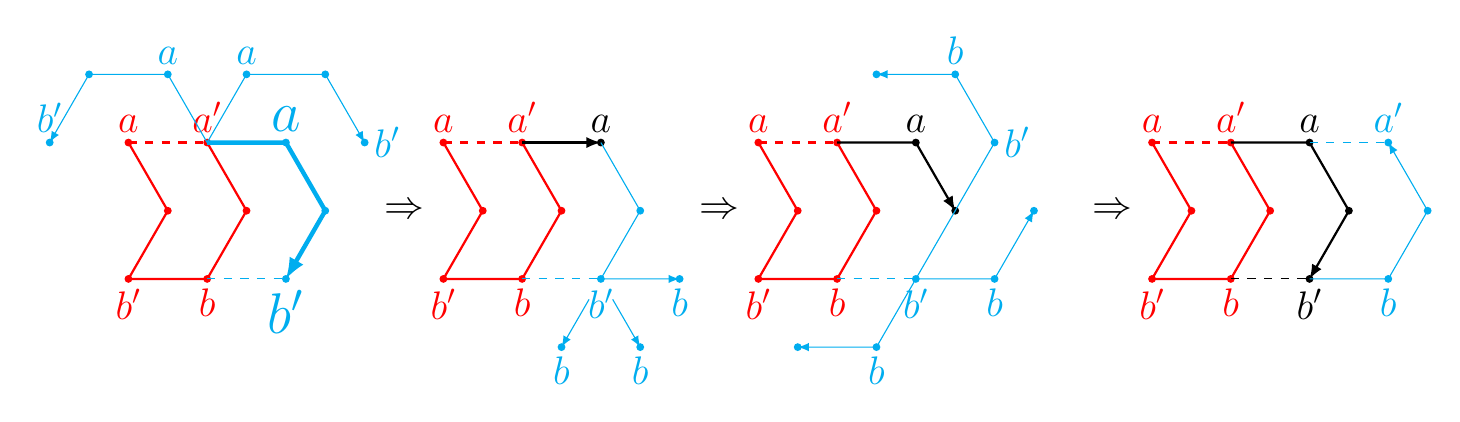
\begin{tikzpicture}
\tikzstyle{mol} = [fill,circle,inner sep=1pt]

\foreach \x in {0, 4, 8, 13} {
\draw[thick, red] (\x, 0) node[mol] {} node[above] {\Large $a$}
-- ++(300:1) node[mol] {} 
-- ++(240:1) node[mol] {} node[below] {\Large $b'$}
-- ++(0:1) node[mol] {} node[below] {\Large $b$}
-- ++(60:1) node[mol] {} 
-- ++(120:1) node[mol] {} node[above] {\Large $a'$}
;
\draw[thick, dashed,red] (\x, 0) -- ++(0:1);
}

\draw[cyan, -latex] (1, 0) -- ++(120:1) node[mol] {} node[above] {\Large $a$} -- ++(180:1) node[mol]{} -- ++(240:1) node[mol] {} node[above] {\Large $b'$};
\draw[cyan, -latex] (1, 0) -- ++(60:1) node[mol] {} node[above] {\Large $a$} -- ++(0:1) node[mol] {} -- ++(300:1) node[mol] {} node[right] {\Large $b'$};
\draw[ultra thick, cyan, -latex] (1, 0) -- ++(0:1) node[mol] {} node[above] {\huge $a$} -- ++(300:1) node[mol] {} -- ++(240:1) node[mol] {} node[below] {\huge $b'$};

\draw[dashed, cyan] (0,0)++(300:2) -- ++(0:1);

\draw (3,0)++(300:1) node {\Large $\Rightarrow$};
\draw (7,0)++(300:1) node {\Large $\Rightarrow$};
\draw (12,0)++(300:1) node {\Large $\Rightarrow$};


\draw[thick, -latex] (5, 0) -- ++(0:1) node[mol] {} node[above] {\Large $a$};

\draw[cyan, -latex] (6, 0) -- ++(300:1) node[mol] {} -- ++(240:1) node[mol] {} node[below] {\Large $b'$} -- ++(0:1) node[mol] {} node[below] {\Large $b$};
\draw[cyan, -latex] (5,0)++(300:2)++(240:0.3) -- ++(240:0.7) node[mol] {} node[below] {\Large $b$};
\draw[cyan, -latex] (5,0)++(300:2.3) -- ++(300:0.7) node[mol] {} node[below] {\Large $b$};
\draw[dashed, cyan] (4,0)++(300:2) -- ++(0:1);


\draw[thick, -latex] (9, 0) -- ++(0:1) node[mol] {} node[above] {\Large $a$}
-- ++(300:1) node[mol] {}
;
\draw[cyan, -latex] (10,0)++(300:1) -- ++(240:1) node[mol] {} node[below] {\Large $b'$}
-- ++(240:1) node[mol] {} node[below] {\Large $b$}
-- ++(180:1) node[mol] {}
;
\draw[cyan, -latex] (9,0)++(300:2) -- ++(0:1) node[mol] {} node[below] {\Large $b$} -- ++(60:1) node[mol] {};
\draw[cyan, -latex] (10,0)++(300:1) -- ++(60:1) node[mol] {} node[right] {\Large $b'$}
-- ++(120:1) node[mol] {} node[above] {\Large $b$}
-- ++(180:1) node[mol] {}
;
\draw[cyan,dashed] (8,0)++(300:2) -- ++(0:1);

\draw[thick, -latex] (14, 0) -- ++(0:1) node[mol] {} node[above] {\Large $a$}
-- ++(300:1) node[mol] {}
-- ++(240:1) node[mol] {} node[below] {\Large $b'$}
;
\draw[dashed] (13,0)++(300:2) -- ++(0:1);
\draw[cyan, -latex] (14,0)++(300:2) -- ++(0:1) node[mol] {} node[below] {\Large $b$}
-- ++(60:1) node[mol] {}
-- ++(120:1) node[mol] {} node[above] {\Large $a'$}
;
\draw[cyan,dashed] (15,0) -- ++(0:1);

\end{tikzpicture}}
\caption{Progression of a glider by distance 1.}
\label{fig:glider}
\vspace*{-3mm}
\end{wrapfigure}
%\end{figure}

%\begin{example}\label{ex:glider}
%A motif called the \emph{glider} explains well how oritatami systems behave. 

Let us provide an example of cyclic DOS that folds into a motif of great use called the \textit{glider}. 
Let $\Sigma = \{a, a', b, b', \bullet\}$. 
Consider a delay-3 OS whose transcript $w$ is a repetition of $a \bullet b' b \bullet a'$ and whose rule set is $\mathcal{H} = \{(a, a'), (b, b')\}$, making $\bullet$-beads inert. 
Its seed, colored in red in Fig.~\ref{fig:glider}, can be elongated by the fragment of the first three beads $w[1..3] = a \bullet b'$ in various ways, only three of which are shown in Fig.~\ref{fig:glider} (left). 
Only the third bead, $b'$, can form a new h-interaction, with the $b$ in the seed (according to $\mathcal{H}$, the first $a$ is also capable of binding, with $a'$, but the sole $a'$ around is just ``too close''). 
For the $b{-}b'$ interaction, the fragment must be folded as bolded in Fig.~\ref{fig:glider} (left). 
According to this most stable folding, the first bead $w[1] = a$ is stabilized to the east of the previous bead, and then the bead $w[4] = b$ is transcribed. 
The next two beads $w[2], w[3]$ are stabilized as illustrated one after another, but we can easily see that the bolded elongation dominates even their stabilization. 
It suffices to observe that neither $w[4]$ nor $w[5]$ can form any new h-interaction. 
When $w[4] = b$ is transcribed (after $w[1]$ is stabilized), $b'$-beads around are either too far or too close  (recall that $w[4]$ cannot interact with $w[3] = b'$). 
In addition, $w[5]$ is inert. 
Thus, they cannot override the bolded ``decision.''
It is easily induced inductively that gliders of arbitrary ``flight distance'' can be folded. 

Gliders also provide a medium to propagate 1-bit at arbitrary distance as the position of their last beads, which is determined by the height (top or bottom) of the first bead and a flying distance.  
%The height (top or bottom) of the first bead determines whether the last bead is stabilized top or bottom after flying a given distance.
For instance, the glider in Fig.~\ref{fig:glider} launches top and thus its last bead (the $a'$) also comes top after traveling the distance 2.
The OS we shall propose exploits this information-carrying capability.

Denote the points in $\mathbb{R}^2$ that correspond to vertices of $\mathbb{T}$ by $\mathbb{Z}_\bigtriangleup^2$. 
A \textit{shape} $S$ is a set of points on the triangular grid. 
For an integer $c \ge 1$, let $Rhomb_c = \{(x, y) \in \mathbb{Z}_{\bigtriangleup}^2 \mid x, y \le c\}$.
Let $S' = \{(cx, cy) \mid (x, y) \in S\}$. 
The \textit{$c$-rhombus scaling} of $S$ is the union over all $\vec{p} \in S'$ of sets of points $Rhomb_c + \vec{p} = \{\vec{v} \in \mathbb{R}^2 \mid \mbox{$\vec{v} = \vec{r} + \vec{p}$ for some $\vec{r} \in Rhomb_c$}\}$.
%The \textit{$c$-rhombus scaling} of a shape $S$ is a shape obtained by expanding the distance between the points in $S$ equally by $c$ to obtain another shape $S'$ and replacing each point $\vec{p} \in S'$ by the rhombus whose sides are of length $c$. 
Let $\diamondsuit_c(S)$ be the $c$-rhombus scaling of $S$. 
We say that an OS $\Xi$ \textit{weakly folds} (or ``self-assembles'') $\diamondsuit_c(S)$ if every terminal assembly of $\Xi$ puts at least one bead in $Rhomb_c + \vec{p}$ for all $\vec{p} \in S$ and no bead in $Rhomb_c + \vec{q}$ for all $\vec{q} \not\in S$. 


%--------------------------------------------------------------------------------------------------------
	\section{Folding the $n$-bit Heighway dragon}
%--------------------------------------------------------------------------------------------------------

We propose a generic design of DOS that allows us to fold an arbitrary finite portion $P[j_1 .. j_2]$ of the slanted Heighway dragon. 
Let $n = \min\{m \mid j_2 < 2^m\}$. 
Independently of $j_1, j_2$, both delay and arity are set to 3 and 567 bead types with a fixed rule set $\mathcal{H}$ are employed (some of the bead types might be saved but not easily due to the NP-hardness of minimizing the number of bead types \cite{HanKim2017}). 
The design also challenges to make the resulting DOS cyclic. 
Otherwise, one could simply implement left and right-turn modules and concatenate their copies according to the (non-periodic) sequence $P$. 
However, it is highly unlikely that an OS for the infinite Heighway dragon, if any, could adopt this approach in order to be describable by a finite mean. 
Such a ``hardcoding'' also goes against the spirit of algorithmic self-assembly. 

\begin{figure}[tb]
\includegraphics[width=\linewidth]{Figs/seed_sample2.png}
\caption{The seed for the 3-bit Heighway dragon that starts at $j_1 = 100_2$.}
\label{fig:seed}
\end{figure}

The initial count $i = j_1$ is encoded on the seed in its binary representation $b_n b_{n-1} \cdots b_1$ as: 
\begin{equation}\label{eq:turner_output}
	{\tt 499 \east 500 \east 501 \east 506 \east 507 \east \mbox{$\bigodot_{k = n}^2$} (w_{t, b_k} \east 350 \east 351 \east (356 \east 357 \east)^6) w_{t, b_1}} 
%	& & \ {\tt 350 \east 351 \east 356 \east 357 \east 316 \east 317 \se}
\end{equation}
where ${\tt w_{t, 0} = 338 \east 339 \east 344 \east 345}$ and ${\tt w_{t, 1} = 346 \east 347 \east 348 \east 349}$. 
Upon this seed, a periodic transcript is folded into the dragon $P[j_1..j_2]$. 
Its period is semantically divided into six \textit{modules} as $C D_v T C D_h T$, where 
\begin{itemize}
\item $C$ is called a \textit{counter module}, which increments $i$ by 1 and propagates it; 
\item $D_v$ and $D_h$ are called a \textit{DFAO module}, which computes $P[i]$ and interprets it properly (this issue of interpretation shall be discussed in the next paragraph); 
\item $T$ is called a \textit{turner module}, which makes a turn according to the interpretation. 
\end{itemize}
The first $C$ and $D_v$ modules fold into a vertical line segment, while the second $C$ and $D_h$ fold into the next line segment, which is guaranteed to be horizontal since vertical and horizontal segments alternate on the Heighway dragon. 
The DFAO modules $D_v, D_h$ differ only in their way to interpret their intermediate outcome $P[i]$. 
The slanted dragon involves two types of left turn as well as two types of right turn: acute and obtuse. 
Observe that after (slanted) vertical line segments, the dragon turns left obtusely and right acutely, whereas after horizontal ones, it turns left acutely and right obtusely. 
Therefore, it suffices for $D_v$ and $D_h$ to compute $P[i] \in \{{\rm L}, {\rm R}\}$ in the same way and $D_v$ interprets L as O and R as A, while $D_h$ interprets L as A and R as O. 

\begin{figure}[tb]
\centering
\includegraphics[width=0.8\linewidth]{Figs/dragon_vol5.png}
\caption{
Folding of one segment plus turn of the Heighway dragon, flow of information through it, and the two ways of collision avoidance between two turns.
}
\label{fig:abst_dragon}
\end{figure}

Before explaining the modules, one issue intrinsic to the folding by OS should be pointed. 
It rises when the dragon makes a turn where it has already turned before. % that is, when two turns share a point. 
By definition, OSs are not allowed to put a bead anywhere occupied by another bead. 
Being scaled sufficiently large, a rhombus corresponding to a point affords two turning modules, which otherwise collide, as long as they fold into an L-shape (Figs.~\ref{fig:heighway6_oritatami}, \ref{fig:abst_dragon}). 
A turning module has its three bifurcator submodules direct further folding obtusely one after another guided by the signal O from the previous DFAO module, as colored in yellow in Figs.~\ref{fig:abst_dragon}, \ref{fig:PFS}, \ref{fig:change_route}, or acutely one after another by A, as colored in green, and folds into two L-shape conformations. 
Note that two turns at a point are both acute or both obtuse. 

Having outlined the generic design, now we explain how the design implements an OS for a specific target portion $P[j_1 .. j_2]$, or more precisely, how the modules $C, D_v, D_h, T$ and their submodules are implemented, interlocked with each other, and collaborate. 
The length of $C, T$, or more precisely, of their transcript, are of length $O(n^2)$ while $D_v, D_h$ are of length $O(n)$. 
Thus, the period of the OS is of length proportional to $n^2$. 

Each of these modules consists of small submodules, say, with several dozens of beads. 
Submodules implement various ``functions'' each of which is ``called'' in proper \textit{environments}, i.e., the beads already placed around the tip of the transcript acting as the memory in the computation. 
The conformation that a submodule folds deterministically in a ``valid'' environment corresponds to the function to be called then. 
These ``expected'' conformations are called \textit{bricks}, as they are the bricks upon which the whole folding is built. 
In order to describe the OS' behavior at submodule level, \textit{brick automata} are employed. 
They enumerate all the pairs of an environment to be encountered and the brick to be folded there as well as transitions among them. 
Using a simulator developed for \cite{HaKiOtSe2016}, we verified all the brick automata, which can be found in Sects.~\ref{ap_subsect:DFAO_module_BA}, and \ref{ap_subsect:Turner_module_BA}. 


\paragraph{Counter module} is borrowed from \cite{GeMeScSe2016} with technical modification to let it operate in the dynamics \eqref{eq:cotranscriptional_folding}, which is more prevailing \cite{HanKim2017,HaKiOtSe2016,OtaSeki2017} though less tractable. 
We hence leave all its details to the Appendix (Sect.~\ref{sect:appendix_counter_module}), and just describe its input and output. 
It takes the current count $i$ formatted as \eqref{eq:turner_output}, which is fed by the seed or by the previous turner module, increments the count by 1 unless it is preceded by the seed, and outputs the resulting count in its binary representation $a_n a_{n-1} \cdots a_1$ in the following format:
\begin{equation}\label{eq:counter_output}{\tt 
	44 \east 45 \east 46 \east 51 \east 52 \east \mbox{$\bigodot_{k = n}^2$} (w_{c, a_k} \east (75 \east 76 \east)^5 51 \east 52 \east) w_{c, a_1}
}\end{equation}
where ${\tt w_{c, 0} = 57 \east 58 \east 63 \east 64 \east 69 \east 70}$ and ${\tt w_{c, 1} = 65 \east 66 \east 67 \east 68 \east 69 \east 70}$. 

\paragraph{DFAO modules $D_v, D_h$} receive the current count $i$ in the format \eqref{eq:counter_output} from the previous counter module, compute $P[i]$, and interpret it as A or O properly. 
$D_v$ and $D_h$ then output the interpretation along with the count $i$ in the following formats, respectively: 
\begin{eqnarray}
& & {\tt \mbox{$\bigodot_{k=n}^2$} (w_{d, a_k} \east (52 \east 51 \east)^7) w_{d, a_1} \east 52 \east 51 \east 200 \east 199 \east w_{dv, P[i]}} \label{eq:Dv_output}\\
& & {\tt \mbox{$\bigodot_{k=n}^2$} (w_{d, a_k} \east (52 \east 51 \east)^7) w_{d, a_1} \east 52 \east 51 \east 311 \east 310 \east w_{dh, P[i]}} \label{eq:Dh_output}
\end{eqnarray}
where ${\tt w_{dv, L} = 198 \east 197}$, ${\tt w_{dv, R} = 194 \east 193}$, ${\tt w_{dh, L} = 305 \east 304}$, and ${\tt w_{dh, R} = 309 \east 308}$.

\begin{figure}[tb]
\includegraphics[width=\linewidth]{pics/abst_DFAO.png}
\caption{Submodule-level abstraction of the folding of DFAO module.}
\label{fig:abst_dfao}
\end{figure}

What the DFAO in Fig.~\ref{fig:heighway_dragon} really does for computing $P[i]$ is to search for the first 0 from the LSB and check whether it is followed by 0 ($P[i] = {\rm R}$) or by 1 ($P[i] = {\rm L}$). 
See Fig.~\ref{fig:abst_dfao}. 
$D_v$ employs the six submodules: Dzig1, Dzag1, Dzig2, Dzag2, PFS, and $\mathrm{AO}_v$ (resp.~$\mathrm{AO}_h$), which are interleaved by spacers, as well as those that guide the transcript into two zigzags and one more zig. 
The first zigzag is for the search, the second zigzag is for the check, and at the beginning of the third zig, as shown in Fig.~\ref{fig:PFS}, $\mathrm{AO}_v$ interprets the output L of PFS as O and R as A, while $\mathrm{AO}_h$ interprets them the other way around otherwise. 

\begin{wrapfigure}{r}{0.65\linewidth}
\vspace*{-5mm}
\centering
\includegraphics[width=\linewidth]{Figs/DFAO-zig1.png}  
\caption{The four bricks of Dzig1: (top) Dzig1-1 and Dzig1-f0; (bottom) Dzig1-20 and Dzig1-21.}
\label{fig:DFAO-zig1}
\vspace*{-3mm}
\end{wrapfigure}

In the first zig, $n$ Dzig1s detect the first 0 collaboratively in two phases. 
See Fig.~\ref{fig:DFAO-zig1} for all the bricks of Dzig1 with the corresponding environments. 
Phase 1 is to copy all the 1's prior to the first 0 and Phase 2 is to copy all the bits after the 0. 
Dzig1 knows which phase it is in by the relative position where it starts folding to the input above (far in Phase1, close in Phase 2). 
In Phase 1, Dzig1's certainly fold into the brick Dzig1-1. 
At the first 0, a Dzig1 rather folds into Dzig1-f0 brick, ending at the top in order to transition to Phase 2. 
Each of the remaining Dzig1 folds into either Dzig1-20 or Dzig1-21, copying all the remaining bits. 
Interleaving spacers are implemented as a glider (see Sect.~\ref{sect:preliminaries}), hence capable of propagating 1bit (far/close) on which phase the system is in. 
In the first zag, $n$ copies of Dzag1 reformat and propagate 0's, 1's, and the first 0 using three bricks in Fig.~\ref{fig:Dzag1}.

\begin{figure}[tb]
\centering
\caption{The five bricks of Dzag2: (top) Dzag2-L0, Dzag2-L1, and Dzag2-T1; (bottom) Dzag2-R0 and Dzag2-R1. 
The first and second halves are diverted to implement the body-rgy and body-gx submodules of the turner module, respectively.}
\label{fig:Dzag2}
\end{figure}

In the second zig, $n$-copies of the submodule Dzig2 check whether the first 0 is followed (being read from LSB) by 0 or 1, in a similar manner to the search in the first zig. 
They usually take one of the two bricks Dzig2-0 and Dzig2-1 to copy 1's and 0's, which start and end at the bottom (see Fig.~\ref{fig:Dzig2}).
At the encounter to the first 0, a Dzig2 folds into a special brick Dzig2-f0 and ends rather at the top. 
The next Dzig2, if any, starts folding at the top so that it takes the special brick Dzig2-0f0 if the first 0 is followed by 0 or Dzig2-1f0 if it is follwed by 1. 
Recall the reading 1 here is a necessary and sufficient condition for the DFAO to transition to $q_2$, that is, $P[i] = L$. 
Dzig2-1f0 exposes a marker $q_2$ downward. 
These bricks ends at the bottom so that the remaining bits are copied by the ordinary bricks Dzig2-0 and -1. 
The second zag starts at the bottom and copy 0's and 1's by the two bricks of Dzag2 (top left and center in Fig.~\ref{fig:Dzag2}) until a Dzag2 encounters the 1 marked by $q_2$, if any. 
At the encounter, the Dzag2 folds into the special brick Dzag2-T1 and changes the ending position to the top, letting the remaining Dzag2 rather fold into the bricks Dzag2-R0 and -R1 for copying, which end at the top. 
As such, the second zag can feed $P[i]$ to PFS as the position of its first bead. 

\paragraph{Turner module}

%--------------------------------------------------------------------------------------------------------
	\bibliographystyle{plain}
	\bibliography{heighway_CIAA2018}
%--------------------------------------------------------------------------------------------------------

%--------------------------------------------------------------------------------------------------------
	\newpage
	\appendix
%--------------------------------------------------------------------------------------------------------

%--------------------------------------------------------------------------------------------------------
	\section{Module automaton}
%--------------------------------------------------------------------------------------------------------

\begin{figure}[h]
\centering
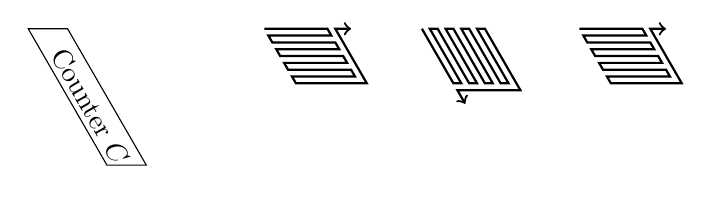
\begin{tikzpicture}

\draw (0, 0) -- ++(0:0.5) -- node[below, sloped] {Counter $C$} ++(300:2) -- ++(180:0.5) -- cycle; 

\foreach \x in {3, 7} {
%\draw (\x, 0) -- ++(0:0.8) -- ++(300:0.8) -- ++(180:0.8) -- cycle;
\draw[thick, ->] (\x, 0) -- ++(0:0.8) -- ++(300:0.1) -- ++(180:0.8) -- ++(300:0.1)
-- ++(0:0.8) -- ++(300:0.1) -- ++(180:0.8) -- ++(300:0.1)
-- ++(0:0.8) -- ++(300:0.1) -- ++(180:0.8) -- ++(300:0.1)
-- ++(0:0.8) -- ++(300:0.1) -- ++(180:0.8) -- ++(300:0.1)
-- ++(0:0.9) -- ++(120:0.8) -- ++(0:0.2)
;
}

\foreach \x in {5} {

\draw[thick, ->] (\x, 0) 
-- ++(300:0.8) -- ++(0:0.1) -- ++(120:0.8) -- ++(0:0.1)
-- ++(300:0.8) -- ++(0:0.1) -- ++(120:0.8) -- ++(0:0.1)
-- ++(300:0.8) -- ++(0:0.1) -- ++(120:0.8) -- ++(0:0.1)
-- ++(300:0.8) -- ++(0:0.1) -- ++(120:0.8) -- ++(0:0.1)
-- ++(300:0.9) -- ++(180:0.8) -- ++(300:0.2)
;
}

\end{tikzpicture}
\caption{Module automaton}
\label{fig:module_automaton}
\end{figure}

%--------------------------------------------------------------------------------------------------------
	\section{Counter module}
	\label{sect:appendix_counter_module}
%--------------------------------------------------------------------------------------------------------

One period of the transcript of the $n$-bit counter module is the concatenation of the following submodules: 
\begin{itemize}
\item $n$ submodules $C_{HA}$; the half-adder; 
\item $n-1$ submodules $C_{SPzig}$ interleaved between the 
half-adders; 
\item Submodule $C_{LT}$; the left-turner; 
\item $n$ submodules $C_{F}$, the formatter; 
\item $n-1$ submodules $C_{SPzag}$ interleaved between the formatters; 
\item Submodule $C_{RT}$; the right-turner.
\end{itemize}


\begin{figure}[htb]
\vspace*{-5mm}
\centering
\includegraphics[width=\linewidth]{Figs/counter_zig.png}
\caption{All conformations of the half-adder.
The first and third are diverted to implement the body-lpx2 component of the turning module. 
}
\label{fig:half-adder}
\end{figure}


%--------------------------------------------------------------------------------------------------------
	\subsection{Transcript}
%--------------------------------------------------------------------------------------------------------

%--------------------------------------------------------------------------------------------------------
	\section{DFAO module}
	\label{sect:appendix_DFAO_module}
%--------------------------------------------------------------------------------------------------------

%--------------------------------------------------------------------------------------------------------
	\subsection{Bricks}
	\label{ap_subsect:DFAO_module_bricks}
%--------------------------------------------------------------------------------------------------------

\begin{figure}[htb]
\centering
%\includegraphics[width=\linewidth]{}
\caption{The three bricks of Dzag1: Dzag1-f0, Dzag1-0, and Dzag1-1.}
\label{fig:Dzag1}
\end{figure}

\begin{figure}[htb]
\centering
%\includegraphics[width=\linewidth]{}
\caption{The five bricks of Dzig2: (top) Dzig2-1, Dzig2-0, Dzig2-f0, (bottom) Dzig2-0f0 and Dzig2-1f0. }
\label{fig:Dzig2}
\end{figure}

%--------------------------------------------------------------------------------------------------------
	\subsection{Brick automata}
	\label{ap_subsect:DFAO_module_BA}
%--------------------------------------------------------------------------------------------------------

The DFAO module is designed at the level of submodule based on the five brick automata shown in Figs.~\ref{fig:brick_automaton_Dzig1}, \ref{fig:brick_automaton_Dzag1}, \ref{fig:brick_automaton_Dzig2}, \ref{fig:brick_automaton_Dzag2}, and \ref{fig:brick_automaton_Dzig3}. 
The labels B and T of transitions stand for that the previous submodule (glider) ends at the bottom and at the top, respectively. 

\begin{figure}[ht]
\centering
\includegraphics[width=\linewidth]{Figs/D-zig1_brick.pdf}
\caption{The brick automaton for the first zig of DFAO module.}
\label{fig:brick_automaton_Dzig1}
\end{figure}

\begin{figure}[ht]
\centering
\includegraphics[width=\linewidth]{Figs/D-zag1_brick.pdf}
\caption{The brick automaton for the first zag of DFAO module.}
\label{fig:brick_automaton_Dzag1}
\end{figure}

\begin{figure}[ht]
\centering
\includegraphics[width=\linewidth]{Figs/D-zig2_brick.pdf}
\caption{The brick automaton for the second zig of DFAO module.}
\label{fig:brick_automaton_Dzig2}
\end{figure}

\begin{figure}[ht]
\centering
\includegraphics[width=\linewidth]{Figs/D-zag2_brick.pdf}
\caption{The brick automaton for the second zzg of DFAO module.}
\label{fig:brick_automaton_Dzag2}
\end{figure}

\begin{figure}[ht]
\centering
\includegraphics[width=\linewidth]{Figs/D-zig3_brick.pdf}
\caption{The brick automaton for the third zig of DFAO module.}
\label{fig:brick_automaton_Dzig3}
\end{figure}

%--------------------------------------------------------------------------------------------------------
	\section{Turner module}
	\label{ap_sect:Turner_module}
%--------------------------------------------------------------------------------------------------------

%--------------------------------------------------------------------------------------------------------
	\subsection{Brick automata}
	\label{ap_subsect:Turner_module_BA}
%--------------------------------------------------------------------------------------------------------

\end{document}
